\lab{Algorithms}{B-Splines}{B-Splines}
Though B\'{e}zier curves are good for a variety of things, they have certain limitations.
\begin{itemize}
\item As the number of control points increases it becomes very expensive to compute the points on the curve.
\item Changes in the placement of a single control point affect the shape of the entire curve.
\item Since a change in any control point affects the entire curve, it is necessary to recompute the entire curve to account for a change in a single control point.
\item As the number of points increases, individual points have progressively less affect on the portions of the curve that lie nearest to them.
\end{itemize}

B-Splines are an ideal way to answer these limitations.
A B-Spline is somewhat similar to a piecewise B\'{e}zier curve.

\section*{B-Spline Basis Functions}

In the previous lab we introduced a way to represent B\'{e}zier curves as a linear combination of Bernstein Polynomials.
We discussed the convenient property that the coefficient of each Bernstein polynomial for the B\'{e}zier curve formed from a given control point is simply the control point itself.
This is a useful property.

\begin{figure}
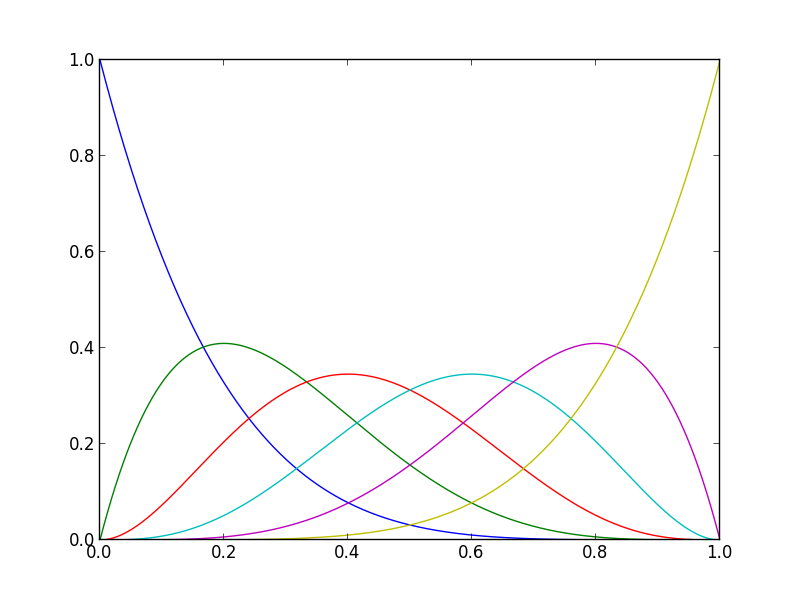
\includegraphics[width=\textwidth]{bernstein_basis}
\caption{5th degree Bernstein basis functions}
\end{figure}

B-splines are a generalization of B\'{e}zier curves which allow us to use piecewise basis functions.
We usually choose basis functions that are zero on most of the domain so that, at any given parameter value, we only have to consider a few of the basis functions to compute the value of a spline
Choosing basis functions that are zero on significant portions of the domain makes it so that we do not have to recompute the entire curve when we change only one control point.
It also makes it so that the curve is easier to manipulate, since local changes in control points only change a portion of the spline curve.

We would like to be able to do this without loosing the useful properties of B\'{e}zier curves.
Using basis functions of any sort guarantees that each point of the curve will be a linear combination of the control points.
It would be best if we could make it so that this curve has the convex hull property (i.e. that it lies within the area bounded by the outermost control points).
B\'{e}zier curves also allow easy computation of their derivatives, so we would hope that B-Splines would allow this as well.
One of the largest constraints we need is that the curve we are forming be continuous with a given number of continuous derivatives.
The construction of the B-Spline Basis functions takes all of these factors into account.

There are a number of ways the B-Spline basis functions can be defined.
A common approach is to use recursion.
Let $t = \lbrace t_0, t_1, ... , t_l \rbrace$ be a nondecreasing sequence of real numbers.
$t$ is called the knot vector.
The $t_i$ are called the knots.
Note that each $t_i$ is not necessarily distinct.
$N_{i,k}(x)$, the $i$'th B-Spline basis function of degree $k$ is defined as:

\begin{equation*}
N_{i,0}(x) =
\begin{cases}
1 & \text{if } t_i \leq x < t_{i+1} \\
0 & \text{otherwise}
\end{cases}
\end{equation*}

\begin{equation*}
N_{i,k}(x) = \frac{x - t_i}{t_{i+k} - t_i} N_{i,k-1}(x) + \frac{t_{i + k + 1} - x}{t_{i + k + 1} - t_{i + 1}} N_{i+1,k-1}(x)
\end{equation*}

This is known as the Cox-De Boor recursion formula.
This algorithm is the De Boor algorithm.
When implemented properly, this algorithm is both fast and numerically stable.
Some simple basis functions are shown in Figure \ref{fig:bspline_basis}.

\begin{figure}
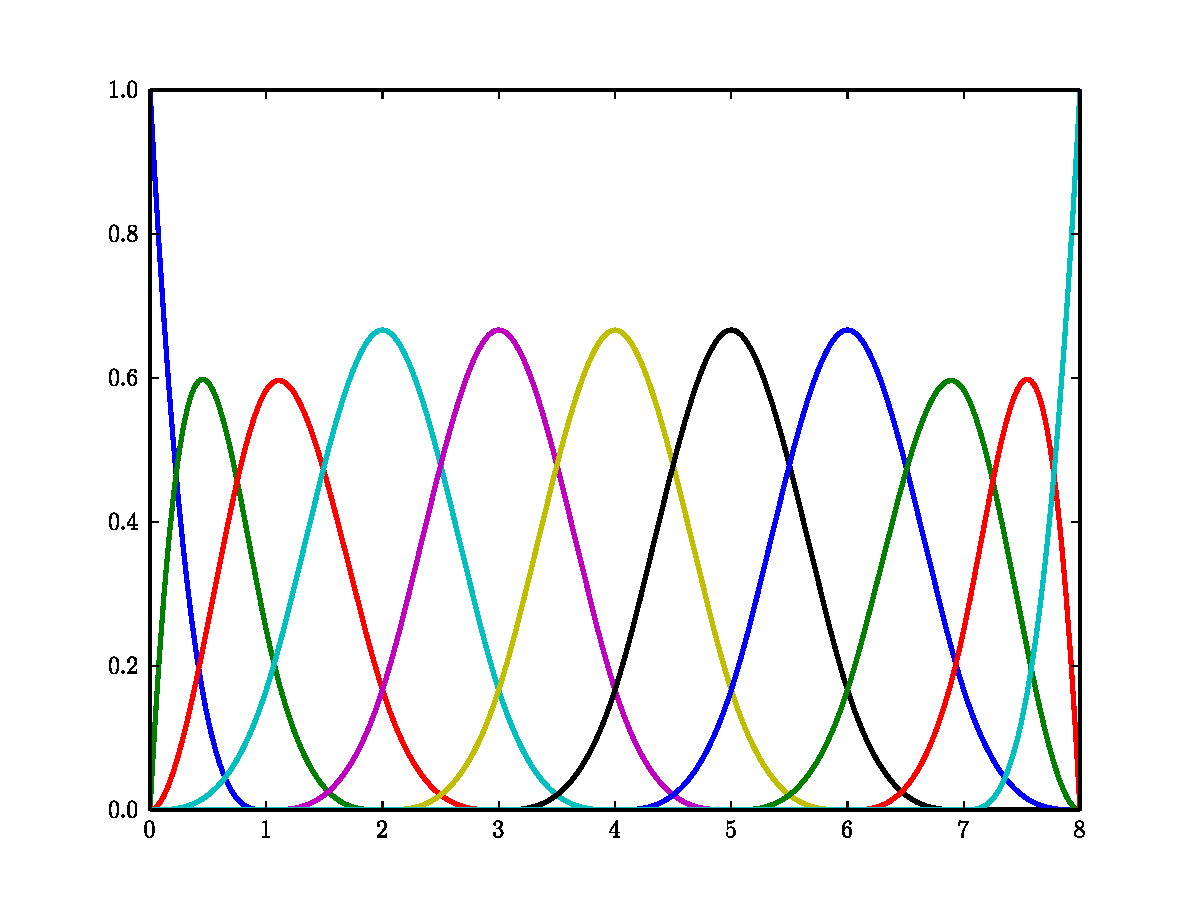
\includegraphics[width=\textwidth]{bspline_basis.pdf}
\caption{B-spline basis functions that are only nonzero on a portion of the given interval.}
\label{fig:bspline_basis}
\end{figure}

Finding the point of a spline at a given parameter value $x$ is done in the same way it was using the Bernstein basis for B-splines.
Where, $P_i$ are the control points, $N_{i,k}$ are the basis functions of degree $k$, and there are $n$ control points , we have that the spline $B$ of degree $k$ can be written
\[B\left(x\right) = \sum_{i=0}^n P_i N_{i,k}\left(x\right)\]

Notice that we defined $t$ to be nondecreasing, which means some $t_i$ may be repeated.
When programming this algorithm as it is currently written, be careful to avoid division by zero.
Whenever we get the indeterminate form $\frac{0}{0}$ or any other sort of division by $0$, we must replace it with zero.

Also note that $N_{i,0}$ is a step function which is zero except on $[t_i, t_{i+1})$.
The other basis functions are piecewise polynomials of degree $k$ that are only nonzero on $[t_{i-k}, t_{i+1+k})$.
This is nice because computation of a set of basis functions requires only a knot vector $t$ and a degree $k$, so we can predefine basis functions before we know the actual positions of the control points.

\begin{warn}
When performing the computation of each of the terms in the De Boor Algorithm, you should very careful about division by $0$.
Whenever division by $0$ occurs in either term, you should replace the value for \emph{that specific term} by $0$.
This should be done for each term independently so that, if you are using NumPy's float types, a value of \li{inf} or \li{nan} does not propagate through the recursion in the algorithm.
You can test to see if a floating point number has a value of \li{nan} or \li{inf} using the functions \li{math.isnan} and \li{math.isinf} or \li{numpy.isnan} and \li{numpy.isinf}.
This can also be done by checking to see if the denominator is $0$ before performing division.
\end{warn}

\begin{problem}
Use the De Boor algorithm to write a recursive python function to evaluate a b-spline basis function for some $x$ between the maximum and minimum of a given knot vector $t$.
\end{problem}

Upon considering the computation involved in the previous problem, we see that this recursion, particularly for higher order splines, involves a massive amount of repetitive calculation.
Many of the performance costs can be avoided by rewriting the algorithm using explicit loops and avoiding unnecessary computations.

\begin{comment}
% These comments and this problem could be one way to expand this lab later on.
% Depending on how long the lab is, we will probably want to give them pseudocode for this version of the algorithm.

First, notice that for splines of order $2$ and higher, we actually compute the values of some splines multiple times.
A simple way to avoid this is to figure out which of the 0-order splines we will actually use in our computation, compute them all, then compute all the needed splines of order 1, 2, etc.

There is also some redundant computation in the computation of the coefficients used at each stage of the recursion.
This can be eliminated by using good control structure and a temporary variable.

We will label the left and right coefficients in the formula $L$ and $R$ respectively, so we have $L(i, k, x) = \frac{x - t_i}{t_{i + k} - t_i}$ and $R(i, p, u) = \frac{t_{i + k + 1} - x}{t_{i + k + 1} - t_{i + 1}}$.
Notice that $L(i + 1, k, x) = 1 - R(i, k, x)$.
We can eliminate much of the duplicate computation by computing the new left hand side coefficient the iteration before we actually need it.
This avoids nearly all the repeated computation.

\begin{problem}
Write a function that uses loops instead of recursion to compute the values for all the b-spline basis functions of a given power $k$ for a given array of $t$ values.
Return the answer as a two dimensional array with the results for each polynomial stored in each of the rows of the array.
\end{problem}

It is worth noting that you can remove further excess computation when evaluating a single function and even further when evaluating a single function at a single point.
This can be done by figuring out in advance which of the $N_{i,k}$ will be nonzero and only iterating over those terms.
This approach may or may not be faster depending on the form of the problem.

\end{comment}

Scipy has some built in functions and a built in class for B-splines.
They are all part of the scipy.interpolate package.

As of SciPy 14, \li{scipy.interpolate} also includes the \li{BPoly} class that allows for easy computation of the basis functions for a B-spline.

Several of the functions built in to SciPy are wrappers around the Fortran package FITPACK.
One such example is the function \li{scipy.interpolate.splev}.
This function is used to evaluate a spline with knot vector $t$, basis function coefficients $c$, and degree $k$ at a set of points $x$.
The calling convention for this function is \li{splev(x, (t, c, k))}.
If $c$ is a multi-dimensional array, the function is applied to each row of $c$.
This is equivalent to using each column of $c$ as a control point in a higher dimension.

The package \li{scipy.interpolate} also includes several routines designed for easy interpolation with b-splines.
It also has routines designed for integration and differentiation of B-splines.

\begin{problem}
Use \li{scipy.interpolate.splev} to generate a plot of a b-spline with control points in $\mathbb{R}^2$ at equally spaced points along the edge of a circle.
Make your control points start and end at the point $\left(1, 0\right)$.
Generate the same plot with your own implementation of the De Boor's algorithm.

Use the following knot vector (where $m$ some positive integer and $k$ is the degree of the desired spline):
\begin{lstlisting}
t = np.array([0]*(k) + range(m) + [m]*(k+1))
\end{lstlisting}
This knot vector will give you $k + m$ different nonzero basis functions on the interval $\left[0, m\right]$.
You will have to include an extra column at the end of your array of control points since this knot vector gives an extra basis function that is equal to $0$.
\end{problem}
